\chapter{Análisis de requerimientos}
\label{cap:corpus}

El primer paso en la construcción de cualquier sistema de software, incluyendo los sistemas de generación de lenguaje natural, es realizar un análisis de requerimientos y a partir de estos generar una especificación inicial para el sistema. Para el análisis de requerimientos, se seguirá el enfoque sugerido por Reiter y Dale~\cite{reiter_dale} en el cual se propone realizar un corpus de textos de ejemplo y a partir de ellos obtener los requerimientos para el trabajo.

\section{Corpus de descripciones}                 

Según la definición de la RAE~\cite{dicrae}, un corpus es un \emph{``conjunto lo más extenso y ordenado posible de datos o textos científicos, literarios, etc., que pueden servir de base a una investigación''}. En particular, el corpus utilizado para la construcción de un sistema de NLG estará formado por un conjunto de ejemplos de datos de entrada junto a la correspondiente salida (texto en lenguaje natural) para cada uno de estos. En nuestro caso, la entrada será un grupo de clases de prueba (en lenguaje Z) junto a las designaciones correspondientes a la especificación testeada, mientras que la salida estará formada por descripciones en lenguaje natural de las clases de prueba antes mencionadas. En lo posible, el corpus de textos deberá cubrir todo el rango de textos que esperan ser producidos por el sistema de NLG; éste debería cubrir los casos más frecuentes, así como los casos más inusuales que pudieran ocurrir.

%~\footnote{Una vez recolectada una colección inicial de textos de ejemplo, es posible que sea necesario aplicar algunas modificaciones sobre ésta. Esto se puede deber a que algunos de los textos recolectados resulten técnicamente implosibles de generar y sea necesarios removerlos del corpus, que existan diferentes variantes correspondientes a la misma entrada de texto y requiramos resolver posibles conflictos, textos que puedan ser mejorados y puedan ser modificados, etc. Llamaremos corpus objetivo al resultado de aplicar al corpus inicial todas las modificaciones antes mencionadas (de ser necesarias).}
Siguiendo la metodología propuesta por Reiter y Dale, para construir el corpus que se utilizará a lo largo de todo el trabajo se deberá elaborar, en primera instancia, un \emph{corpus inicial} y luego, de ser necesario, se deberá trabajar el mismo a fin de confeccionar un \emph{corpus objetivo} que será con el que finalmente se trabajará. Para construir un \emph{corpus inicial} se debe recolectar un conjunto lo suficientemente amplio de ejemplos que debería ser representativo de la variedad de textos que se desea generar. Luego una persona capacitada (en nuestro caso alguien capaz de leer esquemas Z y con un alto conocimiento del dominio de aplicación) deberá describir en lenguaje natural los ejemplos antes mencionados. Esta colección de ejemplos y descripciones de los mismos constituirá nuestro \emph{corpus inicial}. Es posible que esta recopilación requiera algunas modificaciones, por ejemplo: podría ocurrir que alguno de los textos resulten técnicamente imposibles de generar y sea necesarios removerlos del corpus, también podrían existir diferentes variantes correspondientes a la misma entrada de texto y deberíamos resolver los posibles conflictos, etc. Llamaremos, finalmente, \emph{corpus objetivo} al resultado de aplicar las modificaciones necesarias al \emph{corpus inicial}. Este \emph{corpus objetivo} es el que se utilizará para sustentar muchas de las decisiones que se tomarán a lo largo de este trabajo. Además, podría ser de utilidad\footnote{Esto no está contemplado dentro del alcance de este trabajo, pero como veremos en el capítulo \ref{cap:conclusion}, podría ser tenido en cuenta en trabajos futuros.} para realizar una evaluación de nuestro sistema una vez desarrollado, comparando los textos generados por la implementación realizada con las descripciones del corpus realizadas por la persona especializada.

En el apéndice~\ref{ape:corpus} podemos encontrar los textos incluidos en el corpus utilizado para este trabajo. Para elaborar el mismo, se ha recolectado una colección de clases de prueba generadas con \emph{Fastest} a partir de distintas especificaciones y luego se escribió manualmente cada una de las descripciones para las mismas. En este proceso, se intentó abarcar todo el rango de textos que se espera que nuestro sistema sea capaz de producir, para esto, se ha tenido en cuenta incluir una gran variedad de clases de pruebas de modo que cubran todas las expresiones u operadores de Z contemplados dentro del alcance de este trabajo, considerando también las posibles combinaciones de estas expresiones. Se trabajó también con especificaciones sobre distintos dominios de aplicación a fin de lograr un corpus que sea de utilidad para dar con una solución independiente del dominio de aplicación. En total se han incluido clases de prueba generadas con \emph{Fastest} para 5 especificaciones distintas; del total se escogieron las más significativas para describir en lenguaje natural y se ignoraron aquellas que contenían algún operador no considerado dentro del alcance de este trabajo.


En la figura~\ref{fig:ej_corpus} podemos observar uno de los ejemplos incluidos en el corpus de descripciones utilizado para este trabajo. En este caso la clase de prueba \emph{LookUp\_SP\_1} (generada a partir de la especificación introducida previamente) y las designaciones correspondientes a la especificación en cuestión serán la entrada del sistema de NLG\footnote{Estrictamente hablando, todas las designaciones de la especificación deberían formar parte de la entrada del sistema de NLG. En este caso, se incluyeron sólo las designaciones relevantes a fin de simplificar el ejemplo.}, teniendo como salida la descripción en lenguaje natural presente en el ejemplo.

\begin{figure}[H]
\begin{itemize}
\item \emph{Clase de prueba para operación LookUp}\\
\begin{schema}{LookUp\_ SP\_ 1}\\
 st : SYM \pfun VAL \\
 s? : SYM 
\where
 s? \in \dom st \\
 \dom st = \{ s? \}
\end{schema}

\item \emph{Designaciones SymbolTable}\\

\begin{itemize}[label={--}]
  \item símbolo a buscar $\approx s?$
  \item símbolos cargados en la tabla $\approx \dom st$
\end{itemize}

\bigskip
\item \emph{Descripción en lenguaje natural para LookUp\_SP\_1}\\

\begin{tcolorbox}[colback=gray!5!white,colframe=gray!50!black,
  colbacktitle=gray!75!black,title=LookUp\_SP\_1]
  Se busca un símbolo en la tabla, cuando:
     \begin{itemize}
  	    \item[--]{El símbolo a buscar pertenece a los símbolos cargados en la tabla.}
        \item[--]{El símbolo a buscar es el único elemento de los símbolos cargados en la tabla.} 
     \end{itemize}
\end{tcolorbox}

\end{itemize}
\caption{Corpus de textos}
\label{fig:ej_corpus}
\end{figure}

\section{Análisis del corpus}
\label{sec:corpus_analisis}

En lo que queda de este capítulo nos encargaremos de analizar los ejemplos presentes en el corpus a fin de extraer los requerimientos para nuestro sistema. Este estudio nos ayudará a sustentar muchas las decisiones que se tomarán al realizar el diseño de nuestro sistema de NLG. 

Comenzaremos analizando las clases de prueba generadas por \emph{Fastest} y la correlación entre la estructura de las mismas y la estructura de las descripciones en lenguaje natural. Luego estudiaremos la verbalización de las expresiones Z presentes en las clases de prueba, analizaremos el rol de las designaciones y se dará un conjunto de reglas para describir estas expresiones. Por último se contemplarán cuestiones gramaticales que se deberán tener en cuenta para la realización del sistema.

\section{Estructura de las descripciones}
\label{sec:corpus_descripciones}
Podemos notar que las clases de prueba generadas por \emph{Fastest} se encuentran formadas siempre por conjunciones de predicados atómicos y que a cada uno de estos le corresponde exactamente una oración en lenguaje natural dentro del texto final. Además, estas oraciones dependen exclusivamente del predicado que describen, es decir, éstas no contienen información sobre otros predicados ni hacen referencia a otras frases generadas. En la figura~\ref{fig:ej_test_desc} podemos evidenciar esta correspondencia.

\begin{figure}[H]
\centering
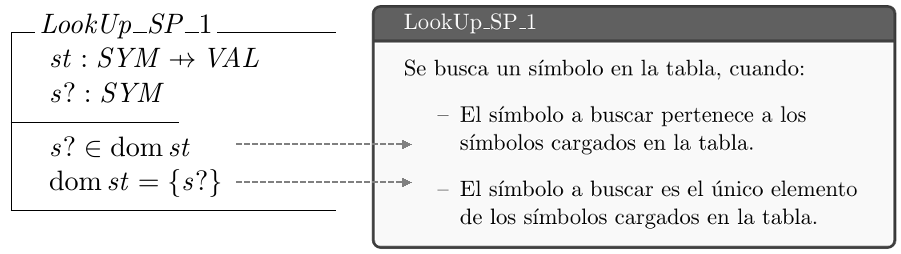
\includegraphics[scale=0.4]{img/ej_test_desc.png}
\caption{Estructura descripciones}
\label{fig:ej_test_desc}
\end{figure}

Además, podemos observar del corpus (apéndice \ref{ape:corpus}) que todas las descripciones de las clases de prueba poseen la misma estructura. En todas se comienza por el nombre de la clase de prueba, seguido por un pequeño detalle de la operación a testear y luego una lista de oraciones encargadas de describir cada uno de los predicados presentes en el cuerpo de la clase de prueba. Conocer la estructura del texto a generar nos será de utilidad para la elaboración del \emph{document plan} (capítulo ~\ref{cap:document_planning}).

\section{Verbalización de expresiones Z}
\label{sec:corpus_verbalizacion}

La tarea de describir un esquema Z correspondiente a una clase de prueba, se puede reducir básicamente a \emph{verbalizar} individualmente cada uno de los predicados atómicos que constituyen el cuerpo del esquema Z. Esta \emph{verbalización} de predicados Z será el desafío principal de este trabajo. Definir con precisión los detalles de ésta será de vital importancia para el desarrollo de las etapas de \emph{microplanning} y \textit{surface realization} de nuestro sistema de NLG (capítulo~\ref{cap:microplanning} y \ref{cap:realization}). En esta sección nos concentraremos especialmente en analizar y especificar la tarea de verbalización.

Podemos notar dos aspectos fundamentales sobre la \emph{verbalización} de expresiones Z. En primer lugar, podemos ver que hay textos que se repiten (con pequeñas variantes, que analizaremos posteriormente) independientemente del dominio de aplicación y que estos surgen a raíz de los operadores de Z presentes en los predicados que se describen. Por otro lado, podemos observar el rol fundamental de las designaciones que posibilitan la introducción de texto dependiente del dominio de aplicación en las descripciones. Consideremos, por ejemplo, las siguientes dos expresiones y sus respectivas descripciones en lenguaje natural, una pertenece al ejemplo de la figura~\ref{fig:ej_corpus} y la otra describe un predicado que forma parte de una clase de prueba para la especificación de un sistema bancario:

\bigskip
\begin{enumerate}
	\item $s? \in \dom st$ $\rightarrow$ \emph{``El símbolo a buscar \textbf{pertenece a}  a los símbolos cargados en la tabla.''}
	\item $num? \in \dom cajas$ $\rightarrow$ \emph{``El número de cuenta del nuevo cliente \textbf{pertenece a} los números de cuenta cargados en el banco.''}
\end{enumerate}
el símbolo a buscar 
\bigskip
Como vemos, el texto \emph{``\textbf{pertenece a}''} aparece en ambas descripciones como resultado de verbalizar el operador $\in$, diferenciándose ambas descripciones en el texto que antecede y sucede al mismo. Por otro lado, estos últimos, bien podrían ser las verbalizaciones de las expresiones que se encuentran a la derecha e izquierda del operador $\in$, respectivamente, por lo que podríamos pensar en una verbalización recursiva sobre la estructura de las expresiones Z. Es posible encontrar estos tipos de patrones en todas las descripciones presentes en el corpus. Esto resulta un buen punto de partida para intentar especificar nuestra tarea de verbalización. En un primer intento, entonces, se definirá la tarea de verbalización en base a los operadores que la componen. Especificaremos esta tarea mediante una función que tomará como entrada una expresión Z y devolverá una descripción en lenguaje natural para la misma. Ésta será recursiva sobre la estructura de las expresiones Z y tendrá tantos casos en su definición como operadores contemplados dentro del alcance de este trabajo (además de las posibles combinaciones de los mismos que puedan resultar de interés y requieran un tratamiento particular). En base al ejemplo anterior, podríamos proponer la siguiente definición para verbalizar el operador $\in$\footnote{Supondremos que el operador $+$ se encargará de realizar una concatenación de \textit{strings} agregando un espacio entre las mismas.}$^{,}$\footnote{El nombre de la función se encuentra primado intencionalmente. Más adelante se presentará la definición final para la función de verbalización que hará uso de \texttt{verb'} como función auxiliar.} :

{
\begin{figure}[H]
\center
$\texttt{verb'} (x \in y) = \texttt{verb}(x) + \text{\emph{``pertenece a''}} + \texttt{verb}(y)$
\end{figure}
}

Como se mencionó anteriormente, para verbalizar términos compuestos se necesitará verbalizar recursivamente las partes que componen a los mismos. En el ejemplo anterior se necesitaría conocer las verbalizaciones de las expresiones $x$ e $y$ para poder obtener una verbalización para $x \in y$.

Retomando el ejemplo de la figura~\ref{fig:ej_corpus}, nos concentraremos en verbalizar la primera expresión de la clase de prueba:

\begin{figure}[H]
\center
$s? \in \dom st$
\end{figure}

En este caso, según la verbalización propuesta anteriormente, podríamos verbalizar la expresión como:

\begin{figure}[H]
\center
$\texttt{verb'} (s? \in \dom st) \rightarrow \texttt{verb}(s?) + \text{\emph{``pertenece a''}} + \texttt{verb}(\dom st)$
\end{figure}

Teniendo que verbalizar $s?$ y $\dom st$. En este caso, ambas expresiones se encuentran designadas, lo que sería de gran ayuda para nuestra tarea de verbalización ya que en estas situaciones podremos construir la descripción en base al texto presente en la designación y sin intentar verbalizar la expresión en base al término Z que la compone. En el ejemplo anterior, no deberíamos intentar verbalizar $\dom st$ como:

\begin{figure}[H]
\center
$\texttt{verb'}(\dom st) \rightarrow \text{\emph{``el dominio''}} + \texttt{verb}(st)$
\end{figure}

\noindent
de hacerlo, estaríamos perdiendo información valiosa para nuestras descripciones contenida en las designaciones ya que las designaciones son nuestra única forma de introducir texto referente al dominio de aplicación en las descripciones. 

En general, para verbalizar una expresión designada, deberemos utilizar el texto presente en las designaciones (en algunos casos, como veremos más adelante, con algunas pequeñas modificaciones, para resolver ciertas cuestiones de concordancia gramatical). Será un requerimiento para nuestra tarea de verbalización, entonces, contemplar en primera instancia si la expresión a describir se encuentra designada antes de intentar describirla en base a los operadores que la componen; de estar designada, se deberá construir una descripción en base a su designación. 

Como se mencionó previamente, el nombre de la función anterior (\texttt{verb'}) fue primado intencionalmente a fin de utilizar esta función como auxiliar para la definición final de la tarea de verbalización. En la figura~\ref{fig:def-verb} se introduce una nueva definición para esta tarea donde se considera la designación de la expresión a verbalizar (si es que se encuentra designada) antes de intentar describir la misma en base a los operadores que la constituyen.

\begin{figure}[H]
\begin{minted}[escapeinside=@@,bgcolor=bg]{haskell}
verb (@$exp$@) = if esta_designada(@$exp$@)
             then designacion(@$exp$@)
             else verb'(@$exp$@)
\end{minted}
\caption{Definición verbalización}
\label{fig:def-verb}
\end{figure}

Como podemos ver en la figura anterior, se hace uso de \texttt{verb'} que será la responsable de generar las verbalizaciones para las expresiones de Z en base a un conjunto de reglas dependientes del operador a describir, como la introducida anteriormente para el caso del operador $\in$. Por otro lado, se abstrae por medio de \texttt{esta\_designada()} la tarea de verificar si una expresión se encuentra designada y mientras que la función \texttt{designacion()} será la encargada de generar una descripción en base a la designación de la expresión a describir. 


Tanto para determinar si una expresión se encuentra designada como para generar una descripción para la misma, deberemos considerar el hecho de que ésta podría estar parametrizada. En particular, para la verbalización de una expresión que se encuentra designada por medio de una designación parametrizada, deberíamos considerar tanto el texto presente en la designación como también la verbalización del argumento parametrizado. Por otro lado, de tratarse de una designación no parametrizada podríamos utilizar el texto tal cual se encuentra en la misma. Por ejemplo, teniendo en cuenta las designaciones introducidas en la figura~\ref{fig:ej_designacion}, obtendríamos la siguiente designación para el término $s?$:

\begin{figure}[H]
\center
$\texttt{designacion}(s?) \rightarrow \text{\emph{``símbolo a buscar''}}$
\end{figure}

\noindent
Por otro lado, si se tratase de un término que concuerda con una designación parametrizada, como $st~s?$, podríamos generar la descripción haciendo uso de su designación y la verbalización del argumento de la siguiente manera: 

\begin{figure}[H]
\center
$\texttt{designacion}(st~s?) \rightarrow \text{\emph{``información asociada a''}} + \texttt{verb}(s?)$
\end{figure}

%\section{Rol de las designaciones}
%\label{sec:corpus_designaciones}

\section{Reglas de verbalización}
\label{sec:corpus_reglas}

En esta sección retomaremos al análisis de la función \texttt{verb'} presentando una especificación para la misma, basada en un conjunto de reglas (similares a la introducida anteriormente para la verbalización del operador $\in$) para la definición por casos de la misma. Luego, en lo que queda de este capítulo nos concentraremos en estudiar, como consecuencia de estas reglas, algunos aspectos gramaticales que deberemos contemplar.

Comenzaremos, a continuación, por completar la definición\footnote{La idea no es que ésta sea una definición final, sino sólo un bosquejo que nos permita analizar los requerimientos que deberán ser contemplados posteriormente, que atenderemos principalmente en las etapas de \textit{microplanning} y \textit{surface realization}.} de \texttt{verb'}, basándonos en los textos presentes en el corpus, incluyendo los casos para todos los operadores considerados dentro del alcance del trabajo, así como las combinaciones más relevantes de los mismos\footnote{Para algunos de estos casos se necesita contemplar el género y número de las verbalizaciones recursivas que lo conforman. En estos casos, nos referiremos al género masculino mediante la letra \emph{M}, y se utilizará \emph{F} para hacer referencia al genero femenino. Por otro lado cuando se haga referencia al número, se utilizará \emph{S} para indicar que el género de un constituyente es singular y \emph{P} en caso de que sea plural.}:
%. Además entraremos más en detalle sobre las tarea de verificar si una expresión se encuentra designada y la generación de un descripción en lenguaje natural para una expresión ya designada.  %Cabe aclarar, que en este caso, tendremos que contemplar si la designación correspondiente es una designación parametrizada. De no ser el caso, el resultado sería exactamente el texto que forma parte de la designación, del contrario, habrá primero que verbalizar el parámetro de la designación, teniendo luego que construir la descripción final a partir del texto de la designación parametrizada y la verbalización del parámetro.
%TODO~\footnote{TODO: aclarar que suponemos que el parámetro debe estar designado?}

\newpage 
\begin{mdframed}[style=codebox]
\begin{minted}[escapeinside=@@]{haskell}

verb' (@$\{exp_1\} = exp_2$@) = verb(@$exp_1$@) + 
                       "es el único elemento de" + 
                       verb(@$exp_2$@)

verb' (@$exp_1 = \{\}$@) = "no hay ningún elemento en" + 
                    verb(@$exp_1$@) 

verb' (@$exp_1 \cap exp_2 = \{\}$@) = verb(@$exp_1$@)  +  
                         "y" +  
                         verb(@$exp_2$@)  +  
                         "no tienen ningún elemento en común"

verb' (@$exp_1 \cap \{exp_2\} = \{\}$@) = verb(@$exp_2$@) +  
                           "no pertenece a" +  
                           verb(@$exp_1$@) 

verb' (@$exp_1 = exp_2$@)
    | (num == S) = verb(@$exp_1$@) + "es igual a" + verb(@$exp_2$@) 
    | (num == P) = verb(@$exp_1$@) + "son iguales a" + verb(@$exp_2$@) 
    where num = numero(verb(@$exp_1$@))

verb' (@$exp_1 \neq \{\}$@) = "existe al menos un elemento en" +  
                    verb(@$exp_1$@) 

verb' (@$exp1 \cap exp2 \neq \{\}$@) = verb(@$exp_1$@)  +  
                         "y" +  
                         verb(@$exp_2$@) +  
                         "tienen al menos un elemento en común" 

verb' (@$exp_1 \neq exp_2$@)
    | (num == S) = verb(@$exp_1$@) + "no es igual a" + verb(@$exp_2$@) 
    | (num == P) = verb(@$exp_1$@) + "no son iguales a" + verb(@$exp_2$@) 
    where num = numero(verb(@$exp_1$@))

verb' (@$exp_1 < exp_2$@) = verb(@$exp_1$@) +  
                     "es menor a" +  
                     verb(@$exp_2$@) 

verb' (@$exp_1 < 0$@)
    | (gen == M) = verb(@$exp_1$@) + "es negativo" 
    | (gen == F) = verb(@$exp_1$@) + "es negativa" 
    where gen = genero(verb(@$exp_1$@))
                                 
verb' (@$exp_1 \leq exp_2$@) = verb(@$exp_1$@) +  
                     "es menor o igual a" +  
                     verb(@$exp_2$@) 

verb' (@$exp_1 > exp_2$@) = verb(@$exp_1$@) +  
                     "es mayor a" +  
                     verb(@$exp_2$@) 

verb' (@$exp_1 > 0$@)  =
    | (gen == M) = verb(@$exp_1$@) + "es positivo" 
    | (gen == F) = verb(@$exp_1$@) + "es positiva" 
    where gen = genero(verb(@$exp_1$@))

verb' (@$exp_1 \geq exp_2$@) = verb(@$exp_1$@) +  
                     "es mayor o igual a" +  
                     verb(@$exp_2$@) 

verb' (@$exp_1 \in exp_2$@)
    | (num == S) = verb(@$exp_1$@) + "pertenece a" + verb(@$exp_2$@) 
    | (num == P) = verb(@$exp_1$@) + "pertenecen a" + verb(@$exp_2$@) 
    where num = numero(verb(@$exp_1$@))

verb' (@$exp_1 \notin exp_2$@)  = 
    | (num == S) = verb(@$exp_1$@) + "no pertenece a" + verb(@$exp_2$@) 
    | (num == P) = verb(@$exp_1$@) + "no pertenecen a" + verb(@$exp_2$@) 
    where num = numero(verb(@$exp_1$@))

verb' (@$exp_1 \subset exp_2$@)
    | (gen == M && num == S) = verb(@$exp_1$@) + 
                               "está incluido en" + 
                               verb(@$exp_2$@) 
    | (gen == M && num == P) = verb(@$exp_1$@) + 
                               "están incluidos en" + 
                               verb(@$exp_2$@) 
    | (gen == F && num == S) = verb(@$exp_1$@) + 
                               "está incluida en" + 
                               verb(@$exp_2$@) 
    | (gen == F && num == P) = verb(@$exp_1$@) + 
                               "están incluidas en" + 
                               verb(@$exp_2$@) 
    where gen = genero(verb(@$exp_1$@))
          num = numero(verb(@$exp_1$@))

verb' (@$\{exp_1, ... , exp_n\} \subset exp_m$@) = verb(@$exp_1$@) +  
                               ", ... , y" +  
                               verb(@$exp_n$@) +  
                               "pertenecen a" +
                               verb(@$exp_m$@)

verb' (@$exp_1 \not\subset exp_2$@)  = 
    | (gen == M && num == S) = verb(@$exp_1$@) + 
                               "no está incluido en" + 
                               verb(@$exp_2$@) 
    | (gen == M && num == P) = verb(@$exp_1$@) + 
                               "no están incluidos en" + 
                               verb(@$exp_2$@) 
    | (gen == F && num == S) = verb(@$exp_1$@) + 
                               "no está incluida en" + 
                               verb(@$exp_2$@) 
    | (gen == F && num == P) = verb(@$exp_1$@) + 
                               "no están incluidas en" + 
                               verb(@$exp_2$@) 
    where gen = genero(verb(@$exp_1$@))
        num = numero(verb(@$exp_1$@))

verb' (@$exp_1 \subseteq exp_2$@) = verb(@$exp_1$@) +  
                    "está incluido o es igual a" +  
                    verb(@$exp_2$@) 

verb' (@$\{exp_1, ... , exp_n\} \subseteq exp_m$@) = verb(@$exp_1$@) +  
                               ", ... , y" +  
                               verb(@$exp_n$@) +  
                               "pertenecen a" +
                               verb(@$exp_m$@)

verb' (@$exp_1 \not\subseteq exp_2$@) = "existe al menos un elemento en" +  
                     verb(@$exp_1$@) +  
                     "que no se está en" +  
                     verb(@$exp_2$@) 

verb' (@$exp_1 \mapsto exp_2$@) = "el par ordenado formado por:" +  
                      verb(@$exp_1$@) +  
                      "y" +  
                      verb(@$exp_2$@) 

verb' (@$\{\}$@) = "el conjunto vacío" 

verb' (@$\{exp_1\}$@) = "el conjunto formado por"  +  
                 verb(@$exp_1$@) 

verb' (@$\{exp_1, ... ,exp_n\}$@) = "el conjunto formado por" +  
                        verb(@$exp_1$@) +  
                        ", ... , y" +  
                        verb(@$exp_n$@) 

verb' (@$exp_1 \cup exp_2$@) = "elementos en" +  
                     verb(@$exp_1$@) +  
                     "y en" +  
                     verb(@$exp_2$@) 

verb' (@$exp_1 \cap exp_2$@) = "elementos en" +  
                    verb(@$exp_1$@) +  
                    "que también se encuentren en" +  
                    verb(@$exp_2$@) 

verb' (@$f~exp_1$@) = verb(@$f$@) +  
                 "aplicada a" +  
                 verb(@$exp_1$@) 

verb' (@$dom(exp_1)$@) = "dominio de" +  
                    verb(@$exp_1$@) 

verb' (@$ran(exp_1)$@) = "rango de" +  
                    verb(@$exp_1$@)  
\end{minted}
\end{mdframed}

Como era de esperarse, podemos notar que, a fin de lograr descripciones más naturales, deberemos contemplar algunas combinaciones entre los distintos términos posibles. Por ejemplo, podemos ver que en el caso de la igualdad entre conjuntos, se propone una descripción para el caso en que uno de los conjuntos esté formado por un único elemento y otra verbalización distinta en el caso de que este conjunto se encuentre vacío.

\section{Aspectos gramaticales}
\label{sec:corpus_gramatica}

Podemos observar que en algunos casos el texto generado por nuestra verbalización puede variar de acuerdo a aspectos gramaticales, en particular, las distintas variantes de nuestras oraciones dependerán del género y número de los constituyentes de las mismas. En estos casos, nos debemos asegurar que las palabras generadas por nuestro sistema concuerden con rasgos gramaticales de, por ejemplo, otra palabra introducida por medio de una designación. Para esto deberemos considerar algunas reglas de \emph{concordancia gramatical}, como la concordancia de número entre el verbo y el núcleo del sujeto para el caso del operador $\in$:


\bigskip
\begin{minted}[escapeinside=@@,bgcolor=bg]{haskell}
verb' (@$exp_1 \in exp_2$@)
     | (num == S) = verb(@$exp_1$@) + "pertenece a" + verb(@$exp_2$@) 
     | (num == P) = verb(@$exp_1$@) + "pertenecen a" + verb(@$exp_2$@) 
     where num = numero(verb(@$exp_1$@))
\end{minted} 

\bigskip
En estos casos, deberemos realizar una análisis del sujeto y según corresponda conjugar correctamente el verbo utilizando, para el ejemplo anterior, deberíamos utilizar el verbo ``\emph{pertenece}'' o ``\emph{pertenecen}'' según corresponda.

Hay algunos casos de la definición anterior en los que el verbo que forma parte del predicado del texto a generar no requieren ningún tratamiento a fin de que el mismo concuerde en número y forma con el sujeto (esto fue contemplado de antemano y no depende de cuestiones externas como podría ser texto introducido por medio de designaciones). Por ejemplo, los siguientes casos:

\bigskip
\begin{minted}[escapeinside=@@,bgcolor=bg]{haskell}
verb' (@$exp_1 = \{\}$@)       = "no hay ningún elemento en" + 
                          verb(@$exp_1$@) 
                                 
verb' (@$exp_1 \cap exp_2 = \{\}$@) = verb(@$exp_1$@)  +  
                         "y" +  
                         verb(@$exp_2$@)  +  
                         "no tienen ningún elemento en común"
\end{minted} 

\bigskip
Por otro lado, podemos observar que las oraciones en las que debemos prestar especial atención a cuestiones de concordancia gramatical resultan oraciones bimembres, todas expresadas en tiempo presente, conformadas de la siguiente manera: 
\begin{figure}[H]
\center
\textbf{sujeto} + \textbf{verbo} + \textbf{objeto}
\end{figure}

\noindent
Como por ejemplo, los siguientes casos:

\bigskip
\begin{enumerate}
 \item \nlgfun{verb'($exp1 \in exp2$)} $\rightarrow$ \textbf{sujeto} + \emph{``pertenece(n)''} + \textbf{objeto}
 \item \nlgfun{verb'($exp1 \subset exp2$)} $\rightarrow$ \textbf{sujeto} + \emph{``está(n) incluido/a(s)''} + \textbf{objeto}
\end{enumerate}

\bigskip
Puntualmente se ha observado que será necesario conjugar el verbo de una oración de forma tal que concuerde con el número del sujeto de la misma. Algo parecido pasa con el atributo en los casos que se utiliza un verbo copulativo en el que se deberá hacer concordar el mismo con número y género del sujeto. Podemos ver que en el ejemplo anterior la palabra \emph{``incluido''} cumple el rol de atributo del verbo copulativo \emph{``estar''} y deberá concordar en número y forma con el sujeto de la oración. 


Otra cuestión que podemos observar a partir de las designaciones documentadas es que, en general para las designaciones no parametrizadas\footnote{Las designaciones parametrizadas son más complejas de trabajar. Éstas estarán formadas generalmente por una oración bimembre que contendrá al parámetro. En el capítulo \ref{sec:verbalizacion_designaciones} retomaremos sobre este tema y estudiaremos en detalle cómo verbalizarlas.}, se utilizan frases nominales para escribir las designaciones. Es decir, presentarán la siguiente estructura:

\begin{figure}[H]
\center
\textbf{[artículo]} + \textbf{sustantivo} + \textbf{[complemento]}
\end{figure}

Como vemos, el artículo puede o no estar presente en las designaciones. Por ejemplo, en ninguna de las designaciones de la figura~\ref{fig:ej_corpus} se incluyeron los artículos, pero fue necesario determinar el artículo indicado (de acuerdo al sujeto) y agregarlos en la descripción. Será un requerimiento, entonces, que nuestro sistema identifique los casos en los que sea necesario agregar el artículo apropiado de forma que concuerde en género y número con el sustantivo. 

Todas estas observaciones sobre la concordancia gramatical entre los constituyentes de nuestras oraciones serán importantes para el desarrollo del realizador lingüístico que estudiaremos en detalle en el capítulo \ref{cap:realization}.

\section{Resumen del capítulo}
En este capítulo se analizaron los aspectos más destacados observados en el corpus de descripciones. Se detallaron los requerimientos necesarios para las distintas etapas de nuestro sistema de NLG. Vimos la estructura de las descripciones que se utilizarán en el capítulo \ref{cap:document_planning} donde estudiaremos la tarea de estructuración del documento, estudiamos la verbalización de expresiones y se presentó una especificación para esta tarea que será de vital ayuda para el desarrollo del \emph{microplanner} que estudiaremos en el capítulo \ref{cap:microplanning}, finalmente observamos algunos aspectos gramaticales que deberemos contemplar para la \textit{surface realization} en el capítulo \ref{cap:realization}.

